\section{Computations}\label{sec:numerics}

\subsection*{Code and meshes}
We use $P_4$ Scott--Vogelius elements with Nitsche's method on the inscribed polygon and strong Dirichlet data on the square $R=(-2.5,2.5)^2$. Divergence is enforced exactly: all ten $P_3$ moments per triangle.

Saddle-point systems are solved by SuperLU \cite{SuperLU} with partial pivoting and three steps of iterative refinement. Over the $148$ production solves ($74$ cases, two methods each), the relative residual is at most $3.8\cdot10^{-15}$ and the discrete divergence at most $7\cdot10^{-11}$ (median $9\cdot10^{-12}$).

The code reproduces the zero-pressure-gradient benchmark of \cite{Cavalcante} to $10^{-5}$ relative on four meshes. It gives $\mu^\ast=60.343$ at $N=20$, against the published $60.338$.

The mesh family has $N$ equal boundary chords and $\rho\approx3.3$, with $\hO$ decreasing from $1.505$ to $0.109$ for $N=16\to256$; rates in $\hO$ and $\hG$ therefore coincide. Rates in the tables are computed between consecutive runs of the full sequence $N=16,24,32,48,64,96,128,192,256$, some of which are omitted from the tables.

\subsection*{Test problems}
\begin{itemize}
\item[\textbf{A}] Scott's benchmark: the shear flow $u=(1-r^{-2})(-y,x)$ with $p\equiv0$, so $G=0$.
\item[\textbf{B$_a$}] $\psi=(r^2-1)^2(x+y^2/2)/10$ and $p=a(x^2y-y+x/2)$, so $G=a(7\pi/8)^{1/2}$: $G=1.658$ for $a=1$ and $165.8$ for $a=100$.
\item[\textbf{P}] Pure pressure: $u\equiv0$, $f=\nabla p$, with $p$ as in B$_1$. $\CNS$ reproduces this exactly ($u_h=0$ and $p_h=p-\pbG(p)$, since $p\in\Pih$); its computed velocity is below $10^{-13}$ in $H^1$. The $\GS$ output is therefore \emph{exactly} the response to the missing traction.
\item[\textbf{C}] $\psi$ as in B, with the non-polynomial pressure $p=e^{x/2}\cos y$. This exercises the term $p^\ast-\pi_hp^\ast$ of Theorem~\ref{thm:D}.
\end{itemize}
Tests A and B were run with $\mu\in\{100,1000,10000\}$ and $N\le192$, plus $N=256$ for $(A,100)$ and $(B_1,100)$, on a 32-core machine (36 minutes in total). Test P (all three $\mu$) and test C ($\mu=100$) were run with $N\le96$ on a 2-core machine.

\begin{figure}[t]
\centering
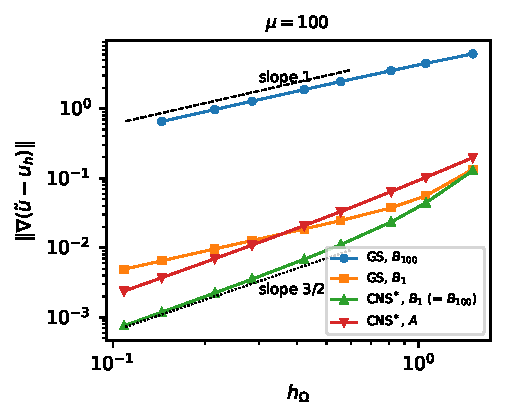
\includegraphics[width=0.48\textwidth]{figures/h1_rates.pdf}\hfill
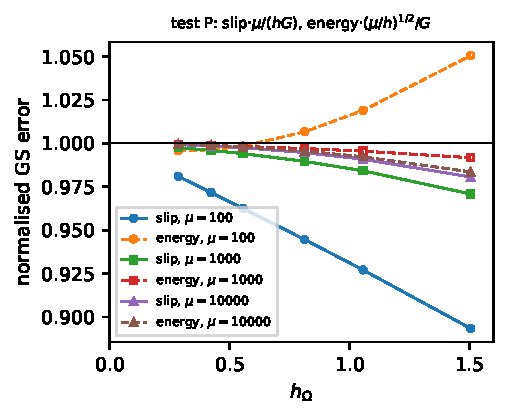
\includegraphics[width=0.48\textwidth]{figures/leading_term.pdf}
\caption{Left: $H^1$ errors at $\mu=100$. $\GS$ has slope $1$ as soon as $G>0$, while $\CNS$ tends to slope $3/2$ independently of the pressure. Right: the normalised slip and energy errors of $\GS$ on test P converge to $1$ (Corollary~\ref{cor:Bp}).}
\label{fig:rates}
\end{figure}

\begin{table}[t]
\centering
\caption{$\CNS$ attains Scott's rate $\hG^{3/2}$ (Theorem~\ref{thm:D}). $H^1$ error, $\mu=100$.}\label{tab:cns}
\begin{tabular}{rrcccc}
\toprule
$N$ & $\hO$ & A & rate & B$_1$ & rate\\
\midrule
32 & 0.813 & $6.41\cdot10^{-2}$ & 1.80 & $2.34\cdot10^{-2}$ & 2.43\\
64 & 0.422 & $2.08\cdot10^{-2}$ & 1.69 & $6.83\cdot10^{-3}$ & 1.76\\
96 & 0.285 & $1.09\cdot10^{-2}$ & 1.64 & $3.54\cdot10^{-3}$ & 1.68\\
128 & 0.215 & $6.96\cdot10^{-3}$ & 1.60 & $2.24\cdot10^{-3}$ & 1.63\\
192 & 0.145 & $3.71\cdot10^{-3}$ & 1.58 & $1.19\cdot10^{-3}$ & 1.60\\
256 & 0.109 & $2.39\cdot10^{-3}$ & 1.56 & $7.58\cdot10^{-4}$ & 1.57\\
\bottomrule
\end{tabular}
\end{table}

\subsection*{Theorem~\ref{thm:D}: $\CNS$}
Table~\ref{tab:cns} gives the $\CNS$ errors. At $N=256$ the energy-norm rate is $1.52$ and the slip rate is $2.02$; the slip carries an extra factor $(h/\mu)^{1/2}$. The $H^1$ rates decrease monotonically toward $3/2$, the geometric term of Lemma~\ref{lem:transposed}. The $\hO^4$ term is invisible at these levels because the geometric term dominates.

The error is independent of the pressure.
\begin{itemize}
\item For polynomial pressures this is structural ($p\in\Pih$). B$_1$ and B$_{100}$ agree to all printed digits wherever both were run ($N\le192$, every $\mu$).
\item With the non-polynomial pressure of test C, the $\CNS$ $H^1$ error differs from that of B$_1$ by a relative $7.9\cdot10^{-7}$, $3.9\cdot10^{-8}$ and $9.7\cdot10^{-9}$ at $N=16$, $64$ and $96$. This is the size of the contribution $\ip{p^\ast-\pi_hp^\ast}{v\cdot n}$, which is of higher order, as Theorem~\ref{thm:D} predicts.
\end{itemize}

\subsection*{Theorems~\ref{thm:A}--\ref{thm:C}: the printed method}
Table~\ref{tab:gs} compares the $H^1$ rates of $\GS$ and $\CNS$ on B$_{100}$.

For the non-polynomial test C at $\mu=100$, the $\GS$ $H^1$ rate from $N=64$ to $96$ is already $1.12$, against $1.68$ for $\CNS$. For the small pressure B$_1$ at $\mu=1000$, $\GS$ still shows $1.51$ at $N=192$. The $(h/\mu)G$ term dominates only once $(h/\mu)G\gtrsim\hG^{3/2}$, which always happens eventually because $\hG^{3/2}$ decays faster. Larger $\mu$ or smaller $G$ delays the crossover but does not remove it.

\begin{table}[t]
\centering
\caption{$\GS$ loses Scott's rate as soon as $G>0$. $H^1$ rate between $N=128$ and $N=192$, test B$_{100}$.}\label{tab:gs}
\begin{tabular}{rcc}
\toprule
$\mu$ & $\GS$ & $\CNS$\\
\midrule
100 & 0.99 & 1.60\\
1000 & 1.00 & 1.56\\
10000 & 1.06 & 1.58\\
\bottomrule
\end{tabular}
\end{table}

\subsection*{Corollary~\ref{cor:Bp}: the leading term}
Table~\ref{tab:P} and Figure~\ref{fig:rates} (right) show the normalised $\GS$ error on test P.
\begin{itemize}
\item The slip and energy ratios converge to $1$. The defect in the slip ratio shrinks with $h/\mu$: at $N=96$ it is $0.019$, $0.0025$ and $0.0007$ for $\mu=10^2$, $10^3$ and $10^4$.
\item The $H^1$ constant is not covered by the corollary. For $\mu=100$ it rises from $2.46$ to $2.71$; for $\mu=10^3$ and $10^4$ it falls, from $2.78$ to $2.77$ and from $3.06$ to $2.79$. This is consistent with a common, $\mu$-independent limit near $2.7$--$2.8$, but the data do not establish one.
\item On test B, $\GS$ itself (B$_1$, $\mu=100$, $N=256$) gives slip and energy ratios $0.995$ and $1.001$.
\item For $\mu=10^4$ with the small pressure B$_1$, $\gamma\hG\approx74\gg G$ at $N=192$, so the hypothesis of the corollary fails. The $\GS$ energy ratio there is about $7.8$, dominated by the geometric error rather than the traction response.
\item The difference $u_{\GS}-u_{\CNS}$ is not a clean proxy for the traction response on test B. It also contains the difference between the two methods on the velocity part, which is $O(\hG^{3/2})$ and non-zero even for test A. Test P removes this.
\end{itemize}

\begin{table}[t]
\centering
\caption{The leading term of Corollary~\ref{cor:Bp}. Normalised $\GS$ error on test P ($G=1.658$), where $e=\ut-u_h$.}\label{tab:P}
\begin{tabular}{rrccc}
\toprule
$N$ & $\mu$ & $\norm{\nabla e}\,\mu/(hG)$ & $\norm{e}_{\Gh}\,\mu/(hG)$ & $\tnorm{e}(\mu/h)^{1/2}/G$\\
\midrule
16 & 100 & 2.464 & 0.894 & 1.051\\
32 & 100 & 2.612 & 0.945 & 1.007\\
64 & 100 & 2.684 & 0.972 & 0.996\\
96 & 100 & 2.708 & 0.981 & 0.996\\
96 & 1000 & 2.770 & 0.998 & 0.999\\
96 & 10000 & 2.790 & 0.9993 & 0.9994\\
\bottomrule
\end{tabular}
\end{table}

\subsection*{Proposition~\ref{prop:penalty}: the penalty study}
The coercivity threshold $\mu^\ast$ on $\Zh$ is the smallest $\mu$ for which the unpivoted symmetric factorisation of $A_\mu+rB^{\mathsf T}M^{-1}B$ has only positive pivots; we locate it by bisection. Table~\ref{tab:thresh} and Figure~\ref{fig:thresh} show the results.

Under refinement at fixed $\rho$, $\gamma^\ast$ increases by $3.4$ ($N=8\to16$), $1.8$ ($16\to32$) and $0.95$ ($32\to64$). The increments roughly halve, which suggests, but does not prove, a limit near $22$.

In part (b) of Table~\ref{tab:thresh}, $\rho$ is varied by coarsening the far field while the boundary layer is held fixed. Then $\mu^\ast$ is linear in $\rho$ over more than a decade, with a constant slope. The threshold is thus set locally at $\Gh$ ($\mu/h\gtrsim c/\hG$), and the $\rho$-scaling is the cost of normalising the penalty by the global $h$.

In practical terms:
\begin{itemize}
\item a safe choice is $\mu\ge25\rho$, that is, $\gamma\ge25$;
\item a fixed $\mu$ fails once the far field is coarsened beyond $\rho\approx\mu/20$.
\end{itemize}
The exact certificate $\lambda\ge9$ on $\cS_3$ and $\cS_4'$ is a local lower bound, consistent with the global $\gamma^\ast\approx18$--$21$.

\begin{table}[t]
\centering
\caption{Coercivity threshold $\mu^\ast$ and $\gamma^\ast=\mu^\ast/\rho$.}\label{tab:thresh}
\small
\textit{(a) Refinement at fixed $\rho$.}\\[2pt]
\begin{tabular}{lcccccccc}
\toprule
$N$ & 8 & 12 & 16 & 20 & 24 & 32 & 48 & 64\\
\midrule
$\rho$ & 3.41 & 3.02 & 3.28 & 3.17 & 3.30 & 3.33 & 3.37 & 3.40\\
$\mu^\ast$ & 50.3 & 51.8 & 59.3 & 60.3 & 63.3 & 66.0 & 69.1 & 70.7\\
$\gamma^\ast$ & 14.7 & 17.1 & 18.1 & 19.1 & 19.2 & 19.9 & 20.5 & 20.8\\
\bottomrule
\end{tabular}\\[6pt]
\textit{(b) Varying $\rho$ through the outer box $(-L,L)^2$.}\\[2pt]
\begin{tabular}{llccccc}
\toprule
 & $L$ & 2.5 & 5 & 10 & 20 & 40\\
\midrule
$N=16$ & $\rho$ & 3.28 & 5.90 & 11.3 & 22.2 & 43.9\\
 & $\mu^\ast$ & 59.3 & 112.1 & 208.0 & 411.5 & 809.3\\
 & $\gamma^\ast$ & 18.1 & 19.0 & 18.4 & 18.5 & 18.4\\
\midrule
$N=32$ & $\rho$ & 3.33 & 5.79 & 10.8 & 21.1 & 41.5\\
 & $\mu^\ast$ & 66.0 & 113.9 & 218.0 & 422.2 & 835.7\\
 & $\gamma^\ast$ & 19.9 & 19.7 & 20.1 & 20.0 & 20.1\\
\bottomrule
\end{tabular}
\end{table}

\begin{figure}[t]
\centering
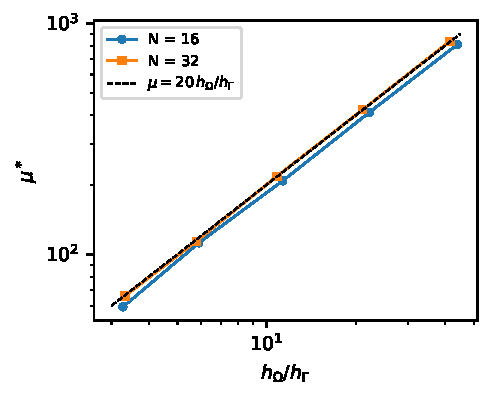
\includegraphics[width=0.48\textwidth]{figures/threshold.pdf}
\caption{Coercivity threshold $\mu^\ast$ against $\rho$ (Table~\ref{tab:thresh}(b)).}
\label{fig:thresh}
\end{figure}

\subsection*{Lemma tests}
We compute exact discrete dual norms, $\sup_v\ell(v)/\norm{\nabla v}$ over $\Zh$ or $\VR$, by a saddle-point solve with the pointwise divergence constraint. Table~\ref{tab:lemma} gives the rates for $N=48\to64$.
\cert{code/lemma\_tests.py 16,24,32,48,64}{logs/lemma\_tests.log}

\begin{table}[t]
\centering
\caption{Exact discrete dual norms; rate in $\hG$ for $N=48\to64$ (positive means decay).}\label{tab:lemma}
\begin{tabular}{llc}
\toprule
Functional & Space & Rate\\
\midrule
$\ip{S}{\dn v}$, $S$ normal & $\Zh$ & $+0.05$ (bounded, $\approx1.75$)\\
$\ip{S}{\dn v}$, $S$ normal & $\VR$ & $-0.52$\\
$\ip{S}{\dn v}$, $S$ tangential & $\Zh$ & $-0.52$\\
$\ip{(\nabla\ut)^{\mathsf T}n}{v}$, tests A / B & $\VR$ & $1.57$ / $1.56$ (Lemma~\ref{lem:transposed}: $3/2$)\\
\bottomrule
\end{tabular}
\end{table}
